% !TeX root = main.tex
% !TEX program = pdflatex

\chapter{Sensores Resistivos}

En este capítulo se estudian los sensores cuyo principio de funcionamiento se basa en la variación de la resistencia eléctrica ($\Delta R$) ante cambios en una magnitud física. Analizaremos desde el modelado físico de potenciómetros y galgas hasta la caracterización de sensores de temperatura (RTD y termistores) y luz (LDR), prestando especial atención a los efectos de carga y las configuraciones de conexión industrial.

\section{Principios Físicos de la Conversión Resistiva}\label{sec:fundamentos_resistivos}

La resistencia de un conductor viene definida por su geometría y su resistividad:
\begin{equation}
    R = \rho \frac{L}{A}
\end{equation}
donde $\rho$ es la resistividad, $L$ la longitud y $A$ el área de la sección transversal. Los sensores resistivos aprovechan la variación de estos parámetros ante estímulos externos:
\begin{itemize}
    \item \emph{Variación geométrica ($\Delta L, \Delta A$)}: Potenciómetros y galgas extensiométricas.
    \item \emph{Variación de resistividad ($\Delta \rho$)}: RTDs, termistores, LDRs y magnetorresistencias.
\end{itemize}
La Figura~\ref{fig:resistencia} ilustra la variación de la resistencia ante cambios en la geometría y la resistividad. En la Figura \ref{fig:resistencia}a se muestra cómo un potenciómetro varía su resistencia al deslizar un contacto móvil, mientras que en la Figura~\ref{fig:resistencia}b se observa cómo una galga extensiométrica cambia su resistencia al estirarse o comprimirse.

\begin{marginfigure}
    \centering
    \shorthandoff{>}
    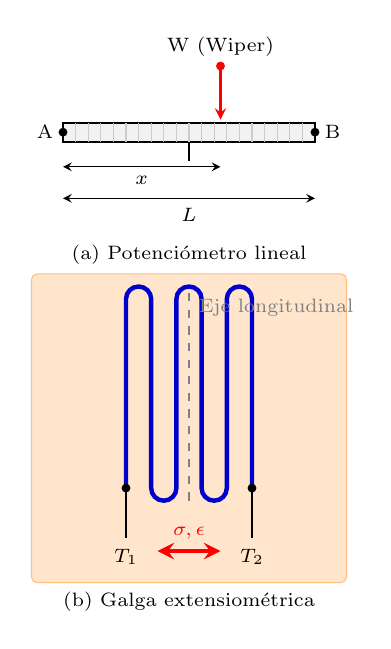
\begin{tikzpicture}[scale=0.8, font=\scriptsize]
        % --- DIBUJO A: POTENCIÓMETRO ---
        \begin{scope}[yshift=0cm]
            % Pista resistiva (rectángulo sombreado)
            \draw[fill=gray!10, thick] (0,0) rectangle (4,0.3);
            \foreach \x in {0.2,0.4,...,3.8} \draw[gray!40] (\x,0) -- (\x,0.3);
            
            % Terminales fijos
            \fill (0,0.15) circle (2pt) node[left] {A};
            \fill (4,0.15) circle (2pt) node[right] {B};
            
            % Contacto móvil (Wiper)
            \draw[thick, red, -stealth] (2.5, 1.2) -- (2.5, 0.35);
            \fill[red] (2.5, 1.2) circle (2pt) node[above, black] {W (Wiper)};
            
            % Cotas de posición
            \draw[<->, >=stealth] (0,-0.4) -- (2.5,-0.4) node[midway, below] {$x$};
            \draw[<->, >=stealth] (0,-0.9) -- (4,-0.9) node[midway, below] {$L$};
            
            % Poner en el centro la etiqueta Potenciometro lineal
            \draw[thick] (2,0) -- (2,-0.3);  
            \node at (2,-1.8) {(a) Potenciómetro lineal};
        \end{scope}

        % --- DIBUJO B: GALGA EXTENSIOMÉTRICA ---
        \begin{scope}[yshift=-5.5cm]
            % Base de la galga (Poliamida)
            \draw[fill=orange!20, draw=orange!50, rounded corners=2pt] (-0.5,-1.5) rectangle (4.5, 3.4);
            
            % Rejilla metálica (Serpentín)
            \draw[ultra thick, blue!80!black] 
                (1,0) -- (1,3) 
                arc(180:0:0.2) -- (1.4,0) 
                arc(-180:0:0.2) -- (1.8,3) 
                arc(180:0:0.2) -- (2.2,0) 
                arc(-180:0:0.2) -- (2.6,3) 
                arc(180:0:0.2) -- (3.0,0);
            
            % Terminales de conexión
            \draw[thick] (1,0) -- (1,-0.8) node[below] {$T_1$};
            \draw[thick] (3.0,0) -- (3.0,-0.8) node[below] {$T_2$};
            \fill (1,0) circle (2pt);
            \fill (3.0,0) circle (2pt);
            
            % Eje de deformación (Esfuerzo)
            \draw[<->, >=stealth, red, ultra thick] (1.5, -1) -- (2.5, -1) node[midway, above] {$\sigma, \epsilon$};
            \draw[dashed, gray] (2, -0.2) -- (2, 3.2) node[pos=0.9, right] {Eje longitudinal};
            
            \node at (2,-1.8) {(b) Galga extensiométrica};
        \end{scope}
    \end{tikzpicture}
    \caption{Representación física de sensores resistivos: (a) Potenciómetro donde la posición $x$ del cursor determina la división de tensión a través del wiper. (b) Galga extensiométrica donde la deformación longitudinal $\epsilon$ altera la resistencia del hilo metálico $\sigma$.}\label{fig:resistencia}
\end{marginfigure}



\section{Potenciómetros de Medida}\label{sec:potenciometros}

En esta sección se analiza el funcionamiento de los potenciómetros como sensores de posición. Se estudia su modelo ideal, la influencia de la carga externa (efecto de carga) y cómo esto afecta la linealidad de la medida.

\subsection{Modelo Ideal y Resolución}

El potenciómetro ideal se modela como una resistencia variable $R(x) = R_{total} \frac{x}{L}$, donde $x$ es la posición del cursor y $L$ la longitud total de la pista resistiva. La salida de tensión por el cursor se obtiene mediante un divisor de tensión: 
\begin{equation}
    V_{out} = V_{in} \frac{R(x)}{R(x) + R_L}
\end{equation}
donde $R_L$ es la resistencia de carga conectada a la salida. En el caso ideal sin carga ($R_L \to \infty$), la salida es lineal con la posición: $V_{out} = V_{in} \frac{x}{L}$.


\subsection{Efecto de Carga y Error de Linealidad}\label{sec:efecto_carga}
% Aquí desarrollaremos el análisis de cómo RL afecta a la medida.
Cuando se conecta una carga $R_L$ a la salida del potenciómetro, el divisor de tensión ya no es ideal y la salida se ve afectada por el efecto de carga, como se muestra en la Figura~\ref{fig:efecto_carga}. La relación entre la salida real y la posición se vuelve no lineal, especialmente cuando $R_L$ es bastante menor que $R(x)$. El error de linealidad introducido por el efecto de carga se puede cuantificar como:
\begin{equation}
    \text{Error} = \frac{V_{out} - V_{ideal}}{V_{ideal}} = \frac{V_{in} \frac{R(x)}{R(x) + R_L} - V_{in} \frac{x}{L}}{V_{in}}
\end{equation}  
\marginnote{\textbf{Efecto de carga:} El efecto de carga es un fenómeno que ocurre cuando la resistencia de carga $R_L$ conectada a la salida del potenciómetro es lo suficientemente baja como para afectar la tensión de salida. Esto provoca una desviación de la respuesta ideal, introduciendo un error de linealidad que se vuelve más pronunciado a medida que $R_L$ disminuye. En aplicaciones donde se requiere alta precisión, es crucial minimizar este efecto utilizando amplificadores de alta impedancia o seleccionando potenciómetros con resistencias totales significativamente mayores que la resistencia de carga.} 
%Figura que ilustra el efecto de carga en la respuesta del potenciómetro, mostrando cómo la salida se desvía de la linealidad ideal a medida que $R_L$ disminuye.
% \begin{marginfigure}
%     \centering
%     \shorthandoff{>}
%     \begin{tikzpicture}
%         \draw[thick] (0,0) -- (4,0);
%         \draw[thick] (0,0) -- (0,2);
%         \draw[thick] (0,2) -- (4,2);
%         \draw[thick] (4,0) -- (4,2);
%         \draw[thick] (2,0) -- (2,2);        
%         \fill (0,0) circle (2pt);        
%         \fill (4,0) circle (2pt);        
%         \fill (0,2) circle (2pt);        
%         \fill (4,2) circle (2pt);        
%         \draw[thick, red, -stealth] (0.5, 1.5) -- (1.5, 0.5) node[midway, above] {$R_L$};
%         \draw[thick, blue, -stealth] (2.5, 1.5) -- (3.5, 0.5) node[midway, above] {$R(x)$};
%         \node at (2, -0.5) {Posición $x$};
%         \node at (2, 2.5) {Tensión de salida $V_{out}$};
%         \node at (2, 1) {Respuesta ideal sin carga};
%         \node at (2, 0.5) {Respuesta con carga $R_L$};
%     \end{tikzpicture}
%     \caption{Ilustración del efecto de carga en un potenciómetro. La curva azul representa la respuesta ideal sin carga, mientras que la curva roja muestra cómo la salida se desvía de la linealidad ideal a medida que la resistencia de carga $R_L$ disminuye.}\label{fig:efecto_carga}
% \end{marginfigure}

El error de linealidad absoluto se define como la diferencia entre la salida real y la ideal: $\epsilon = V_{o,real} - V_{o,ideal}$. El error relativo máximo ocurre aproximadamente en $k \approx 0.67$ (2/3 del recorrido) y se puede aproximar por:
\begin{equation}
    \epsilon_{\max} \approx \frac{4}{27} \frac{R_t}{R_L} \times 100\%
\end{equation}

\begin{marginfigure}[2em]
    \centering
    \shorthandoff{>}
    % --- ESQUEMA DEL CIRCUITO ---
    \begin{tikzpicture}[scale=1]
        % Fuente y Potenciómetro
        \draw (0,0) node[ground]{} to[V, v=$V_i$] (0,3) -- (2,3);
        \draw (2,3) to[R, l=$R_1$] (2,1.5) coordinate (wiper);
        \draw (wiper) to[R, l=$R_2$] (2,0) node[ground]{};
        
        % Conexión a Carga
        \draw (wiper) -- (3.5,1.5) to[R, l=$R_L$] (3.5,0) node[ground]{};
        \draw (3.5,1.5) to[short, -o] (4,1.5) node[right] {$V_o$};
        
        % Etiquetas de resistencia
        \node[left, font=\tiny] at (1.75,2.25) {$(1-k)R_t$};
        \node[left, font=\tiny] at (1.75,0.75) {$k R_t$};
    \end{tikzpicture}
    
    \vspace{1cm}
    
    % --- GRÁFICA DE ERROR ---
    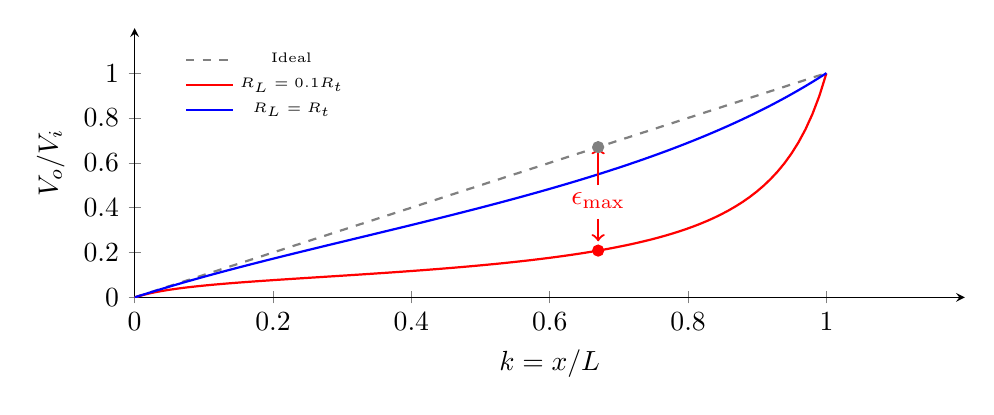
\begin{tikzpicture}
        \begin{axis}[
            width=\linewidth, height=5cm,
            xlabel={$k = x/L$}, ylabel={$V_o/V_i$},
            xmin=0, xmax=1.2, ymin=0, ymax=1.2,
            ytick={0, 0.2, 0.4, 0.6, 0.8, 1}, 
            xtick={0, 0.2, 0.4, 0.6, 0.8, 1},
            %font=\tiny,
            axis lines=left,
            legend style={at={(0.05,0.95)}, anchor=north west, draw=none, font=\tiny}
        ]
            % Respuesta Ideal (Recta)
            \addplot[thick, gray, dashed, domain=0:1] {x};
            \addlegendentry{Ideal};

            % Respuesta con Carga (Rt/RL = 10 para que se note mucho)
            % Formula: x / (1 + x*(1-x)*10)
            \addplot[thick, red, domain=0:1, samples=100] {x / (1 + x*(1-x)*10)};
            \addlegendentry{$R_L = 0.1 R_t$};
            
            % Respuesta con Carga (Rt/RL = 1)
            \addplot[thick, blue, domain=0:1, samples=100] {x / (1 + x*(1-x)*1)};
            \addlegendentry{$R_L = R_t$};
            
            % Marcar el punto de error máximo
            \addplot[only marks, mark=*, red] coordinates {(0.67,{0.67 / (1 + 0.67*(1-0.67)*10)})};
            % ahora sobre la recta ideal
            \addplot[only marks, mark=*, gray] coordinates {(0.67,0.67)};

            \node[red] at (axis cs:0.67,0.43) {$\epsilon_{\max}$};
            % Dibujar una flecha para indicar el error máximo
            \draw[->, thick, red] (axis cs:0.67,0.35) -- (axis cs:0.67,0.25);
            \draw[->, thick, red] (axis cs:0.67,0.5) -- (axis cs:0.67,0.67);

        \end{axis}
    \end{tikzpicture}
    \caption{Efecto de carga. El circuito (arriba) muestra la $R_L$ en paralelo con el brazo inferior. La gráfica (abajo) ilustra cómo la salida se \emph{aplasta} respecto a la ideal, perdiendo linealidad. El eje $y$ representa la relación $V_o/V_i$ y el eje $x$ la posición del cursor.}\label{fig:efecto_carga}
\end{marginfigure}

Ese error se vuelve significativo cuando $R_L$ es pequeño, lo que reduce la resolución efectiva del potenciómetro. Para minimizar este efecto, se recomienda utilizar un amplificador de alta impedancia de entrada o seleccionar un potenciómetro con una resistencia total $R_{total}$ mucho mayor que la resistencia de carga $R_L$. Se utiliza un amplificador operacional en configuración seguidor de tensión para asegurar que la carga no afecte la medida, manteniendo la linealidad y precisión del potenciómetro. eso es debido a que el seguidor de tensión presenta una impedancia de entrada muy alta, lo que minimiza el efecto de carga y permite obtener una salida que sigue fielmente la tensión en el cursor del potenciómetro.

\section{Galgas Extensiométricas (\textit{Strain Gauges})}\label{sec:galgas}

Se estudia el comportamiento de las galgas extensiométricas como sensores de deformación. Se analiza el factor de galga, los tipos de galgas (metálicas y de semiconductor) y cómo la temperatura afecta su respuesta, así como las técnicas de compensación para mitigar estos efectos. Se discuten también las aplicaciones industriales de las galgas en la medición de esfuerzos y deformaciones en estructuras.\marginnote{\textbf{Ejercicio para clase:} 
    Si tenemos un potenciómetro de \SI{10}{\kilo\ohm} y queremos que el error de linealidad por efecto de carga sea inferior al \SI{0.5}{\%}, ¿cuál debe ser la resistencia mínima del sistema de adquisición?     
    \textit{Solución: $R_L > \SI{296}{\kilo\ohm}$.}
}

\subsection{El Factor de Galga ($G$)}
Una galga es un sensor que mide la deformación ($\epsilon$) a través de la variación de su resistencia ($\Delta R$). El factor de galga se define como:
\begin{equation}
    G = \frac{\Delta R / R}{\epsilon}
\end{equation}
Este factor depende del material y la geometría de la galga. Para galgas metálicas típicas, $G \approx 2$, mientras que para galgas de semiconductor puede ser mucho mayor, llegando a valores de $G \approx 100$ o más, debido a la fuerte dependencia de la resistividad con la deformación. La Figura~\ref{fig:factor_galga} muestra la relación entre la deformación y la variación de resistencia para diferentes tipos de galgas, destacando cómo las galgas de semiconductor presentan una respuesta mucho más sensible a la deformación en comparación con las galgas metálicas.

% \begin{marginfigure}
%     \centering
%     \shorthandoff{>}
%     \begin{tikzpicture}
%         \begin{axis}[
%             width=\linewidth, height=5cm,
%             xlabel={Deformación $\epsilon$}, ylabel={Variación de Resistencia $\Delta R / R$},
%             xmin=0, xmax=0.01, ymin=0, ymax=1.0,
%             ytick={0, 0.2, 0.4, 0.6, 0.8, 1.0}, 
%             xtick={0, 0.0025, 0.005, 0.0075, 0.01},
%             axis lines=left,
%             legend style={at={(0.05,0.95)}, anchor=north west, draw=none, font=\tiny}
%         ]
%             % Galga Metálica (G ~ 2)
%             \addplot[thick, blue] {2*x};
%             \addlegendentry{G = 2 (Metálica)};

%             % Galga de Semiconductor (G ~ 100)
%             \addplot[thick, red] {100*x};
%             \addlegendentry{G = 100 (Semiconductor)};
%         \end{axis}
%     \end{tikzpicture}
%     \caption{Relación entre la deformación $\epsilon$ y la variación de resistencia $\Delta R / R$ para galgas metálicas y de semiconductor. Las galgas de semiconductor muestran una respuesta mucho más sensible a la deformación en comparación con las galgas metálicas debido a su mayor factor de galga $G$.}\label{fig:factor_galga}
% \end{marginfigure}

\begin{marginfigure}
    \centering
    \shorthandoff{>}
    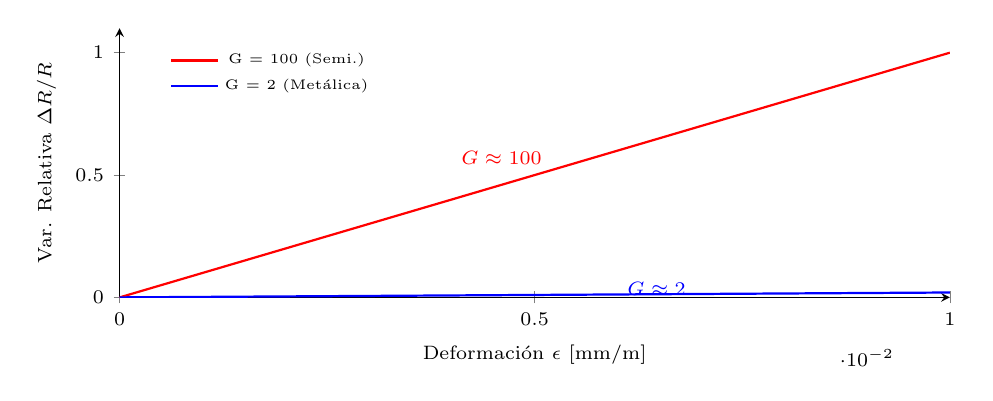
\begin{tikzpicture}
        \begin{axis}[
            width=\linewidth, height=5cm,
            xlabel={Deformación $\epsilon$ [mm/m]}, 
            ylabel={Var. Relativa $\Delta R / R$},
            % Definimos el dominio para que coincida con la vista
            xmin=0, xmax=0.01, 
            ymin=0, ymax=1.1,
            % Formato de números para evitar notación científica amontonada
            xtick={0, 0.005, 0.01},
            xticklabel style={/pgf/number format/fixed, /pgf/number format/precision=3},
            axis lines=left,
            font=\scriptsize,
            legend style={at={(0.05,0.95)}, anchor=north west, font=\tiny, draw=none}
        ]
            % Galga de Semiconductor (G = 100)
            % IMPORTANTE: domain=0:0.01 evita el error "Dimension too large"
            \addplot[thick, red, domain=0:0.01, samples=2] {100*x};
            \addlegendentry{G = 100 (Semi.)};

            % Galga Metálica (G = 2)
            \addplot[thick, blue, domain=0:0.01, samples=2] {2*x};
            \addlegendentry{G = 2 (Metálica)};

            % Nodo explicativo
            \node[red, anchor=south west] at (axis cs:0.004, 0.5) {$G \approx 100$};
            \node[blue, anchor=north west] at (axis cs:0.006, 0.1) {$G \approx 2$};
        \end{axis}
    \end{tikzpicture}
    \caption[Comparativa de sensibilidad entre galgas.]{Comparativa de sensibilidad entre galgas. Nótese que para una deformación de \qty{0.01}{mm/m}, la galga metálica apenas varía un \qty{2}{\percent}, mientras que la de semiconductor llega al \qty{100}{\percent} de variación ($\Delta R = R$).}\label{fig:factor_galga}
\end{marginfigure}

\subsection{Tipos de Galgas: Metálicas y de Semiconductor}
Las galgas metálicas están hechas de aleaciones como Constantán o Karma, que tienen un factor de galga relativamente bajo pero son estables y lineales con la temperatura. Las galgas de semiconductor, por otro lado, utilizan materiales como silicio o germanio, que presentan una alta sensibilidad debido a su fuerte dependencia de la resistividad con la deformación. Sin embargo, las galgas de semiconductor son más susceptibles a la temperatura, poco lineales y requieren técnicas de compensación para mantener la precisión en aplicaciones industriales.

%Usos
Las galgas extensiométricas metálicas se utilizan comúnmente en aplicaciones de ingeniería civil y mecánica para medir esfuerzos en puentes, edificios y maquinaria. Las galgas de semiconductor, debido a su alta sensibilidad, se emplean en aplicaciones donde se requieren mediciones de deformación extremadamente precisas, como en la investigación científica y en la industria aeroespacial.

%MEMS
Las galgas de semiconductor se han miniaturizado en forma de dispositivos MEMS (\textit{Microelectromechanical Systems}), que integran sensores de deformación con circuitos electrónicos en un solo chip, permitiendo aplicaciones avanzadas en monitoreo estructural y biomecánica. Un ejemplo de MEMS es el acelerómetro piezoresistivo como el que semuestra en la Figura~\ref{fig:mems_acelerometro}, que utiliza galgas de semiconductor para medir la aceleración a través de la deformación inducida en las estructuras del dispositivo que como máximo ejempo es el acelerómetro del teléfono móvil, que detecta la orientación del dispositivo y permite funciones como el cambio automático entre modo vertical y horizontal. Las galgas de semiconductor muestran una respuesta mucho más sensible a la deformación en comparación con las galgas metálicas debido a su mayor factor de galga $G$. Las galgas son regiones del propio silicio de la viga que han sido dopadas selectivamente (es decir, con impurezas mediante un proceso de difusion o implantación iónica) para ser piezorresistivas.\marginnote{\textbf{Dopaje y Orientación Cristalina:} El efecto piezorresistivo en el silicio es anisotrópico (depende de la dirección). Dopaje tipo P (Boro): Es el más utilizado en MEMS. Se introducen átomos de Boro (trivalentes) que crean \emph{huecos}. El silicio tipo P es extremadamente sensible a los esfuerzos de cizalla en la dirección cristalográfica <110>, que es la dirección estándar de los brazos en un acelerómetro. Dopaje tipo N (Fósforo/Arsénico): Se introducen electrones en exceso. Aunque también es piezorresistivo, su coeficiente de sensibilidad suele ser menor que el del tipo P para la mayoría de las configuraciones. Existe un compromiso con la catidad de dopaje. Bajo Dopaje: Si ponemos pocos átomos de Boro, el sensor es muy sensible (Factor de Galga $G$ muy alto), pero es inestable con la temperatura. Cualquier cambio térmico altera la resistencia tanto como la deformación. Alto Dopaje (Silicio Degenerado): Si saturamos el silicio con mucho Boro, el sensor se vuelve muy estable térmicamente, pero pierde mucha sensibilidad (el Factor de Galga $G$ baja). La Figura~\ref{fig:zona_dopada} muestra la integración de la galga de semiconductor en el acelerómetro piezoresistivo. Lo que hace que el dopaje sea piezorresistivo es que las impurezas permiten que los cambios en la red cristalina afecten directamente a la nube de electrones/huecos, algo que en un aislante o en un conductor metálico normal no ocurre con tanta intensidad.
} Se colocan sobre la superficie de la viga, lo más cerca posible de las uniones (con el marco, que tambien es de silicio fijo). Si imaginamos la viga como una tabla de trampolín, cuando la masa se mueve, la viga se dobla. El punto donde el silicio se estira y se comprime más (máximo esfuerzo mecánico) es justo en el \emph{encastre}, es decir, donde la viga nace del marco fijo (y también donde se une a la masa). De hecho, para un acelerómetro de alta calidad (puente completo), se suelen poner galgas en ambos extremos de cada viga (una cerca del marco y otra cerca de la masa).

%Figura de un MEMS del acelerómetro piezoresistivo, mostrando cómo las galgas de semiconductor están integradas en la estructura del dispositivo para medir la aceleración a través de la deformación inducida.
\begin{marginfigure}
    \centering
    \shorthandoff{>}
    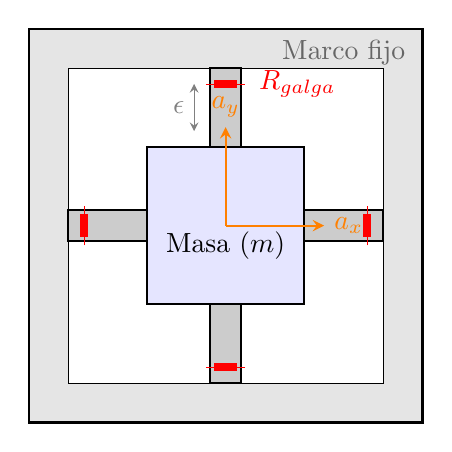
\begin{tikzpicture}[scale=1]
        % Marco exterior (Sustrato de silicio fijo)
        \draw[thick, fill=gray!20] (-2.5,-2.5) rectangle (2.5,2.5);
        \draw[fill=white] (-2,-2) rectangle (2,2); % Hueco grabado
        
        % Masa sísmica (Proof Mass)
        \draw[thick, fill=blue!10] (-1,-1) rectangle (1,1);
        \node at (0,-0.25) {Masa ($m$)};
        
        % Brazos de suspensión (Vigas/Flexures)
        % Arriba
        \draw[thick, fill=gray!40] (-0.2,1) rectangle (0.2,2);
        % Abajo
        \draw[thick, fill=gray!40] (-0.2,-1) rectangle (0.2,-2);
        % Izquierda
        \draw[thick, fill=gray!40] (-1,-0.2) rectangle (-2,0.2);
        % Derecha
        \draw[thick, fill=gray!40] (1,-0.2) rectangle (2,0.2);
        
        % Galgas piezorresistivas (Semiconductoras)
        % Se colocan en los puntos de máximo esfuerzo (unión viga-marco)
        \foreach \x/\y/\r in {0/1.8/0, 0/-1.8/0, -1.8/0/90, 1.8/0/90} {
            \begin{scope}[shift={(\x,\y)}, rotate=\r]
                \fill[red] (-0.15,-0.05) rectangle (0.15,0.05);
                \draw[red, ultra thin] (-0.25,0) -- (0.25,0); % Contactos
            \end{scope}
        }
        
        % Leyendas y etiquetas
        \node[red, anchor=west] at (0.3, 1.8) {$R_{galga}$};
        \node[gray!80!black] at (1.5, 2.2) {Marco fijo};
        
        % Ejes de sensibilidad
        \draw[thick, -stealth, orange] (0,0) -- (0,1.25) node[above] {$a_y$};
        \draw[thick, -stealth, orange] (0,0) -- (1.25,0) node[right] {$a_x$};
        
        % Detalle de flexión
        \draw[<->, >=stealth, gray] (-0.4, 1.2) -- (-0.4, 1.8) node[midway, left] {$\epsilon$};

    \end{tikzpicture}
    \caption[Estructura de un acelerómetro MEMS.]{Estructura de un acelerómetro MEMS. La aceleración desplaza la masa central, deformando las vigas de suspensión. Las galgas de semiconductor (en rojo) integradas en las zonas de máxima flexión detectan la deformación $\epsilon$. El silicio tiene excelentes propiedades mecánicas (no presenta histéresis elástica y es casi tan duro como el acero), lo que permite fabricar sensores de aceleración extremadamente robustos y de bajo coste. }\label{fig:mems_acelerometro}
\end{marginfigure}

\begin{marginfigure}[0em]
    \centering
    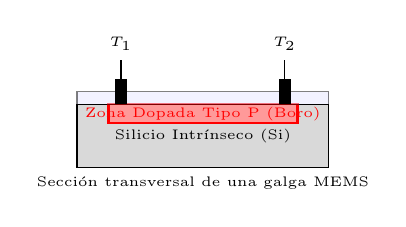
\begin{tikzpicture}[scale=0.8, font=\tiny]
        % Sustrato de Silicio (Bulk)
        \draw[fill=gray!30] (0,0) rectangle (4,1);
        \node at (2,0.5) {Silicio Intrínseco (Si)};
        
        % Zona Dopada (La galga)
        \draw[fill=red!40, draw=red, thick] (0.5,0.7) rectangle (3.5,1);
        \node[red] at (2,0.85) {Zona Dopada Tipo P (Boro)};
        
        % Capa de Pasivación (Óxido)
        \draw[fill=blue!10, opacity=0.5] (0,1) rectangle (4,1.2);
        
        % Contactos de Aluminio
        \fill[black] (0.6,1) rectangle (0.8,1.4);
        \fill[black] (3.2,1) rectangle (3.4,1.4);
        \draw (0.7,1.4) -- (0.7,1.7) node[above] {$T_1$};
        \draw (3.3,1.4) -- (3.3,1.7) node[above] {$T_2$};
        
        \node[below] at (2,0) {Sección transversal de una galga MEMS};

        % Vista de planta

    \end{tikzpicture}
    \caption{Integración de la galga en el silicio. La zona roja es la que cambia su resistividad ante la flexión del sustrato.}\label{fig:zona_dopada}
\end{marginfigure}

Ante una aceleración externa $\vec{a}$, la masa central experimenta una fuerza inercial $\vec{F}=m\vec{a}$. Esta fuerza provoca el desplazamiento de la masa, lo que genera una flexión en las vigas de suspensión. Según la teoría de vigas, el esfuerzo máximo ($\sigma$) se produce en la unión de las vigas con el marco fijo formado por un sustrato de silicio fijo. Las galgas de semiconductor situadas en estos puntos críticos aprovechan su elevado Factor de Galga ($G \approx 100$) para convertir la deformación en una variación de resistencia significativa ($\Delta R/R = G \cdot \epsilon \approx 0.1$). Normalmente, estas cuatro galgas se conectan en una configuración de puente de Wheatstone completo para maximizar la sensibilidad y compensar efectos térmicos no deseados.

\subsection{Influencia de la Temperatura y Compensación}
La temperatura afecta tanto a las galgas metálicas como a las de semiconductor, aunque de manera diferente. En las galgas metálicas, la resistencia varía con la temperatura debido al coeficiente de temperatura de la resistividad ($\alpha$), lo que puede introducir errores en la medida de deformación. En las galgas de semiconductor, la dependencia de la resistividad con la temperatura es aún más pronunciada, lo que puede resultar en errores significativos si no se compensa adecuadamente. Para mitigar estos efectos, se utilizan técnicas de compensación como la conexión en puente de Wheatstone, donde se combinan galgas activas (sujetas a deformación) con galgas de referencia (no deformadas) para cancelar las variaciones debidas a la temperatura. Además, se pueden emplear materiales con bajo coeficiente de temperatura o implementar algoritmos de corrección basados en mediciones de temperatura para mejorar la precisión de las galgas en entornos variables.

\section{Sensores de Temperatura Resistivos (RTD)}\label{sec:rtd}




\subsection{Metales Utilizados: El platino y la Pt100}
\subsection{Ecuación de Callendar-Van Dusen}
\subsection{Configuraciones de Conexión: 2, 3 y 4 hilos}\label{sec:conexion_hilos}
% Vital para instrumentación industrial.
\subsection{Error por Autocalentamiento}

\section{Termistores (NTC y PTC)}\label{sec:termistores}

\subsection{Termistores NTC: Modelo Exponencial y Parámetro $\beta$}
\subsection{Ecuación de Steinhart-Hart}
\subsection{Linealización de la Respuesta NTC}
\subsection{Termistores PTC y aplicaciones de protección}

\section{Sensores de Luz y Campos Magnéticos}\label{sec:otros_resistivos}

\subsection{Fotorresistencias (LDR): Respuesta Espectral}
\subsection{Magnetorresistencias (AMR y GMR)}

\section{Circuitos de Medida: El Puente de Wheatstone}\label{sec:puente_wheatstone}

\subsection{Análisis del Puente Desequilibrado}
\subsection{Configuraciones: Cuarto, Medio y Puente Completo}
\subsection{Linealidad según el tipo de excitación (Voltaje vs. Corriente)}

\section{Resumen de Errores en Sensores Resistivos}\label{sec:errores_resistivos}